%
% hbars.tex
%
\renewcommand{\thisname}{Chart::HorizontalBars}
\section{\thisname}
\name{\thisname}
\file{HorizontalBars.pm}
\requires{Chart::Base, GD, Carp, FileHandle}
\begin{Description}
The class \thisclass creates a chart of horizontally oriented bars.
\thisclass is a subclass of \class{Chart::Base}.
\end{Description}

\example
\begin{figure}[ht]
  \begin{center}
    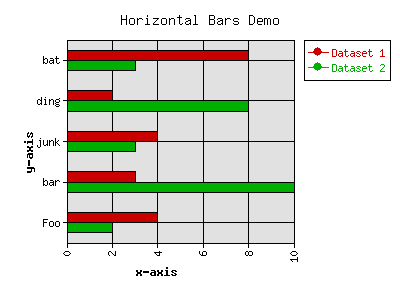
\includegraphics[scale=0.7]{d_hbars4.png}
  \end{center}
  \caption{Chart with horizontal bars}
  \label{fig:hbars}
\end{figure}
\begin{verbatim}
use Chart::HorizontalBars;

$g = Chart::HorizontalBars->new();
$g->add_dataset('Foo', 'bar', 'junk', 'ding', 'bat');
$g->add_dataset(4, 3, 4, 2, 8);
$g->add_dataset(2, 10, 3, 8, 3);

%hash = ( 'title'        => 'Horizontal Bars Demo',
          'grid_lines'   => 'true',
          'x_label'      => 'x axis',
          'y_label'      => 'y axis',
          'include_zero' => 'true',
          'x_ticks'      => 'vertical',
         );
$g->set(%hash);

$g->png("hbars.png");
\end{verbatim}

\constructorblurb{\thisname}

\begin{AttrDecl}{skip\_y\_ticks}
Does the same fo the $y$ axis in a horizontal chart as
\attruse{skip\_x\_ticks} does for other charts. Defaults to 1.
\end{AttrDecl}

\begin{AttrDecl}{spaced\_bars}
Leaves some space between each group of bars when set to \literal{true}. This
usually make it easier to read a bar chart. Default is \literal{true}.
\end{AttrDecl}

\begin{AttrDecl}{y\_axes}
Tells \thisclass where to place the $y$ axis.
\literal{left}, \literal{right} and \literal{both}. Defaults to
\literal{left}.
\end{AttrDecl}
